\let\negmedspace\undefined
\let\negthickspace\undefined
\documentclass[journal]{IEEEtran}
\usepackage[a5paper, margin=10mm, onecolumn]{geometry}
%\usepackage{lmodern} % Ensure lmodern is loaded for pdflatex
\usepackage{tfrupee} % Include tfrupee package

\setlength{\headheight}{1cm} % Set the height of the header box
\setlength{\headsep}{0mm}     % Set the distance between the header box and the top of the text

\usepackage{gvv-book}
\usepackage{gvv}
\usepackage{cite}
\usepackage{amsmath,amssymb,amsfonts,amsthm}
\usepackage{algorithmic}
\usepackage{graphicx}
\usepackage{textcomp}
\usepackage{xcolor}
\usepackage{txfonts}
\usepackage{listings}
\usepackage{enumitem}
\usepackage{mathtools}
\usepackage{gensymb}
\usepackage{comment}
\usepackage[breaklinks=true]{hyperref}
\usepackage{tikz}
\usepackage{tkz-euclide} 
\usepackage{pgfplots}
% \usepackage{gvv}                                        
\def\inputGnumericTable{}                                 
\usepackage[latin1]{inputenc}                                
\usepackage{color}                                            
\usepackage{array}                                            
\usepackage{longtable}                                       
\usepackage{calc}                                             
\usepackage{multirow}                                         
\usepackage{hhline}                                           
\usepackage{ifthen}                                           
\usepackage{lscape}
\begin{document}

\bibliographystyle{IEEEtran}
\vspace{3cm}

\title{11.16.4.9.2}
\author{EE24BTECH11026 - G.Srihaas}
% \maketitle
% \newpage
% \bigskip
{\let\newpage\relax\maketitle}

\renewcommand{\thefigure}{\theenumi}
\renewcommand{\thetable}{\theenumi}
\setlength{\intextsep}{10pt} % Space between text and floats


\numberwithin{equation}{enumi}
\numberwithin{figure}{enumi}
\renewcommand{\thetable}{\theenumi}

\textbf{QUESTION} \\
If 4-digit numbers greater than 5,000 are randomly formed from the digits 0, 1, 3, 5, and 7, what is the probability of forming a number divisible by 5 when the repetition of digits is not allowed?\\

\textbf{SOLUTION} \\
To solve this problem, we need to determine the probability of forming a 4-digit number greater than 5,000 using the digits {0, 1, 3, 5, 7} without repetition, such that the number is divisible by 5.\\

\textbf{Total Valid 4-Digit Numbers}
A 4-digit number greater than 5,000 must start with either 5 or 7. The remaining digits can be any of the remaining digits without repetition.
\begin{itemize}
\item First Digit: 2 choices (5 or 7).
\item Second Digit: 4 choices (excluding the first digit).
\item Third Digit: 3 choices (excluding the first two digits).
\item Fourth Digit: 2 choices (excluding the first three digits).
\end{itemize}
Total valid numbers:
\begin{align}
2 \times 4 \times 3 \times 2 = 48
\end{align}

\textbf{Numbers Divisible by 5}
A number is divisible by 5 if its last digit is either 0 or 5. We consider two cases:\\
\begin{enumerate}
\item  \begin{itemize}
\item Last Digit is 0
\item First Digit: 2 choices (5 or 7).
\item Second Digit: 3 choices (excluding the first digit and 0).
\item Third Digit: 2 choices (excluding the first two digits and 0).
\item Fourth Digit: 1 choice (0).
\end{itemize}
   Total numbers:
   \begin{align}
   2 \times 3 \times 2 \times 1 = 12
   \end{align}

\item
\begin{itemize}
\item Last Digit is 5
\item First Digit: 1 choice (7, since 5 is already used as the last digit).
\item Second Digit: 3 choices (excluding the first digit and 5).
\item Third Digit: 2 choices (excluding the first two digits and 5).
\item Fourth Digit: 1 choice (5).
\end{itemize}
\end{enumerate}

   Total numbers:
   \begin{align}
   1 \times 3 \times 2 \times 1 = 6
   \end{align}

Total numbers divisible by 5:
\begin{align}
12 + 6 = 18
\end{align}

\textbf{Probability Calculation}
The probability $P$ is the ratio of numbers divisible by 5 to the total valid numbers:
\begin{align}
P = \frac{18}{48} = \frac{3}{8} = 0.375
\end{align}\\

The above steps are summarized as follows.\\

\begin{enumerate}

\item Generate All Valid 4-Digit Numbers:
    \begin{itemize}
   \item Generate all combinations of 4-digit numbers starting with 5 or 7.
   \item Ensure no repetition of digits.
    \end{itemize}

\item Check Divisibility by 5:
    \begin{itemize}
    \item For each valid number, check if the last digit is 0 or 5.
    \end{itemize}
\item Count and Calculate Probability:
    \begin{itemize}
   \item Count the total valid numbers and the numbers divisible by 5.
   \item Compute the probability as the ratio of the two counts.
    \end{itemize}     
\end{enumerate}

\begin{figure}[h!]
   \centering
   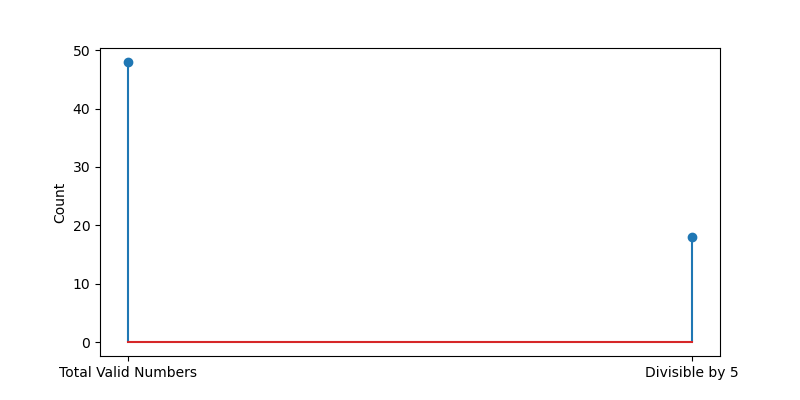
\includegraphics[width=0.6\columnwidth]{figs/fig1.png}
\end{figure}

\begin{figure}[h!]
   \centering
   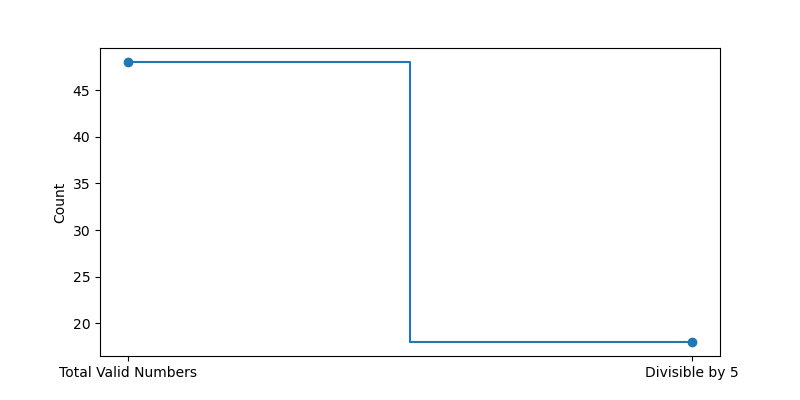
\includegraphics[width=0.6\columnwidth]{figs/fig2.png}
\end{figure}

\end{document}
